\documentclass[1p]{elsarticle_modified}
%\bibliographystyle{elsarticle-num}

%\usepackage[colorlinks]{hyperref}
%\usepackage{abbrmath_seonhwa} %\Abb, \Ascr, \Acal ,\Abf, \Afrak
\usepackage{amsfonts}
\usepackage{amssymb}
\usepackage{amsmath}
\usepackage{amsthm}
\usepackage{scalefnt}
\usepackage{amsbsy}
\usepackage{kotex}
\usepackage{caption}
\usepackage{subfig}
\usepackage{color}
\usepackage{graphicx}
\usepackage{xcolor} %% white, black, red, green, blue, cyan, magenta, yellow
\usepackage{float}
\usepackage{setspace}
\usepackage{hyperref}

\usepackage{tikz}
\usetikzlibrary{arrows}

\usepackage{multirow}
\usepackage{array} % fixed length table
\usepackage{hhline}

%%%%%%%%%%%%%%%%%%%%%
\makeatletter
\renewcommand*\env@matrix[1][\arraystretch]{%
	\edef\arraystretch{#1}%
	\hskip -\arraycolsep
	\let\@ifnextchar\new@ifnextchar
	\array{*\c@MaxMatrixCols c}}
\makeatother %https://tex.stackexchange.com/questions/14071/how-can-i-increase-the-line-spacing-in-a-matrix
%%%%%%%%%%%%%%%

\usepackage[normalem]{ulem}

\newcommand{\msout}[1]{\ifmmode\text{\sout{\ensuremath{#1}}}\else\sout{#1}\fi}
%SOURCE: \msout is \stkout macro in https://tex.stackexchange.com/questions/20609/strikeout-in-math-mode

\newcommand{\cancel}[1]{
	\ifmmode
	{\color{red}\msout{#1}}
	\else
	{\color{red}\sout{#1}}
	\fi
}

\newcommand{\add}[1]{
	{\color{blue}\uwave{#1}}
}

\newcommand{\replace}[2]{
	\ifmmode
	{\color{red}\msout{#1}}{\color{blue}\uwave{#2}}
	\else
	{\color{red}\sout{#1}}{\color{blue}\uwave{#2}}
	\fi
}

\newcommand{\Sol}{\mathcal{S}} %segment
\newcommand{\D}{D} %diagram
\newcommand{\A}{\mathcal{A}} %arc


%%%%%%%%%%%%%%%%%%%%%%%%%%%%%5 test

\def\sl{\operatorname{\textup{SL}}(2,\Cbb)}
\def\psl{\operatorname{\textup{PSL}}(2,\Cbb)}
\def\quan{\mkern 1mu \triangleright \mkern 1mu}

\theoremstyle{definition}
\newtheorem{thm}{Theorem}[section]
\newtheorem{prop}[thm]{Proposition}
\newtheorem{lem}[thm]{Lemma}
\newtheorem{ques}[thm]{Question}
\newtheorem{cor}[thm]{Corollary}
\newtheorem{defn}[thm]{Definition}
\newtheorem{exam}[thm]{Example}
\newtheorem{rmk}[thm]{Remark}
\newtheorem{alg}[thm]{Algorithm}

\newcommand{\I}{\sqrt{-1}}
\begin{document}

%\begin{frontmatter}
%
%\title{Boundary parabolic representations of knots up to 8 crossings}
%
%%% Group authors per affiliation:
%\author{Yunhi Cho} 
%\address{Department of Mathematics, University of Seoul, Seoul, Korea}
%\ead{yhcho@uos.ac.kr}
%
%
%\author{Seonhwa Kim} %\fnref{s_kim}}
%\address{Center for Geometry and Physics, Institute for Basic Science, Pohang, 37673, Korea}
%\ead{ryeona17@ibs.re.kr}
%
%\author{Hyuk Kim}
%\address{Department of Mathematical Sciences, Seoul National University, Seoul 08826, Korea}
%\ead{hyukkim@snu.ac.kr}
%
%\author{Seokbeom Yoon}
%\address{Department of Mathematical Sciences, Seoul National University, Seoul, 08826,  Korea}
%\ead{sbyoon15@snu.ac.kr}
%
%\begin{abstract}
%We find all boundary parabolic representation of knots up to 8 crossings.
%
%\end{abstract}
%\begin{keyword}
%    \MSC[2010] 57M25 
%\end{keyword}
%
%\end{frontmatter}

%\linenumbers
%\tableofcontents
%
\newcommand\colored[1]{\textcolor{white}{\rule[-0.35ex]{0.8em}{1.4ex}}\kern-0.8em\color{red} #1}%
%\newcommand\colored[1]{\textcolor{white}{ #1}\kern-2.17ex	\textcolor{white}{ #1}\kern-1.81ex	\textcolor{white}{ #1}\kern-2.15ex\color{red}#1	}

{\Large $\underline{11a_{199}~(K11a_{199})}$}

\setlength{\tabcolsep}{10pt}
\renewcommand{\arraystretch}{1.6}
\vspace{1cm}\begin{tabular}{m{100pt}>{\centering\arraybackslash}m{274pt}}
\multirow{5}{120pt}{
	\centering
	\includegraphics[width=112pt]{../../../GIT/diagram.site/Diagrams/png/448_11a_199.png}\\
\ \ \ A knot diagram\footnotemark}&
\allowdisplaybreaks
\textbf{Linearized knot diagam} \\
\cline{2-2}
 &
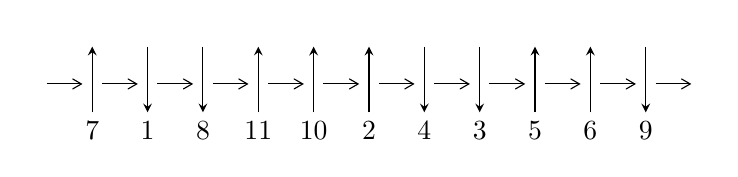
\begin{tikzpicture}[x=20pt, y=17pt]
	% nodes
	\node (C0) at (0, 0) {};
	\node (C1) at (1, 0) {};
	\node (C1U) at (1, +1) {};
	\node (C1D) at (1, -1) {7};

	\node (C2) at (2, 0) {};
	\node (C2U) at (2, +1) {};
	\node (C2D) at (2, -1) {1};

	\node (C3) at (3, 0) {};
	\node (C3U) at (3, +1) {};
	\node (C3D) at (3, -1) {8};

	\node (C4) at (4, 0) {};
	\node (C4U) at (4, +1) {};
	\node (C4D) at (4, -1) {11};

	\node (C5) at (5, 0) {};
	\node (C5U) at (5, +1) {};
	\node (C5D) at (5, -1) {10};

	\node (C6) at (6, 0) {};
	\node (C6U) at (6, +1) {};
	\node (C6D) at (6, -1) {2};

	\node (C7) at (7, 0) {};
	\node (C7U) at (7, +1) {};
	\node (C7D) at (7, -1) {4};

	\node (C8) at (8, 0) {};
	\node (C8U) at (8, +1) {};
	\node (C8D) at (8, -1) {3};

	\node (C9) at (9, 0) {};
	\node (C9U) at (9, +1) {};
	\node (C9D) at (9, -1) {5};

	\node (C10) at (10, 0) {};
	\node (C10U) at (10, +1) {};
	\node (C10D) at (10, -1) {6};

	\node (C11) at (11, 0) {};
	\node (C11U) at (11, +1) {};
	\node (C11D) at (11, -1) {9};
	\node (C12) at (12, 0) {};

	% arrows
	\draw[->,>={angle 60}]
	(C0) edge (C1) (C1) edge (C2) (C2) edge (C3) (C3) edge (C4) (C4) edge (C5) (C5) edge (C6) (C6) edge (C7) (C7) edge (C8) (C8) edge (C9) (C9) edge (C10) (C10) edge (C11) (C11) edge (C12) ;	\draw[->,>=stealth]
	(C1D) edge (C1U) (C2U) edge (C2D) (C3U) edge (C3D) (C4D) edge (C4U) (C5D) edge (C5U) (C6D) edge (C6U) (C7U) edge (C7D) (C8U) edge (C8D) (C9D) edge (C9U) (C10D) edge (C10U) (C11U) edge (C11D) ;
	\end{tikzpicture} \\
\hhline{~~} \\& 
\textbf{Solving Sequence} \\ \cline{2-2} 
 &
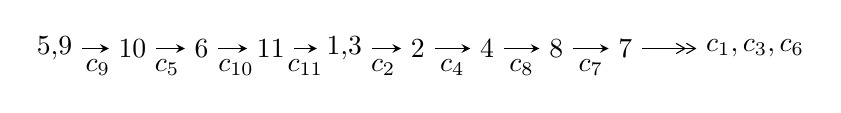
\begin{tikzpicture}[x=25pt, y=7pt]
	% node
	\node (A0) at (-1/8, 0) {5,9};
	\node (A1) at (1, 0) {10};
	\node (A2) at (2, 0) {6};
	\node (A3) at (3, 0) {11};
	\node (A4) at (65/16, 0) {1,3};
	\node (A5) at (41/8, 0) {2};
	\node (A6) at (49/8, 0) {4};
	\node (A7) at (57/8, 0) {8};
	\node (A8) at (65/8, 0) {7};
	\node (C1) at (1/2, -1) {$c_{9}$};
	\node (C2) at (3/2, -1) {$c_{5}$};
	\node (C3) at (5/2, -1) {$c_{10}$};
	\node (C4) at (7/2, -1) {$c_{11}$};
	\node (C5) at (37/8, -1) {$c_{2}$};
	\node (C6) at (45/8, -1) {$c_{4}$};
	\node (C7) at (53/8, -1) {$c_{8}$};
	\node (C8) at (61/8, -1) {$c_{7}$};
	\node (A9) at (10, 0) {$c_{1},c_{3},c_{6}$};

	% edge
	\draw[->,>=stealth]	
	(A0) edge (A1) (A1) edge (A2) (A2) edge (A3) (A3) edge (A4) (A4) edge (A5) (A5) edge (A6) (A6) edge (A7) (A7) edge (A8) ;
	\draw[->>,>={angle 60}]	
	(A8) edge (A9);
\end{tikzpicture} \\ 

\end{tabular} \\

\footnotetext{
The image of knot diagram is generated by the software ``\textbf{Draw programme}" developed by Andrew Bartholomew(\url{http://www.layer8.co.uk/maths/draw/index.htm\#Running-draw}), where we modified some parts for our purpose(\url{https://github.com/CATsTAILs/LinksPainter}).
}\phantom \\ \newline 
\centering \textbf{Ideals for irreducible components\footnotemark of $X_{\text{par}}$} 
 
\begin{align*}
I^u_{1}&=\langle 
2 u^{39}-2 u^{38}+\cdots+4 b-2,\;- u^{38}+17 u^{36}+\cdots+4 a+2,\;u^{40}-2 u^{39}+\cdots+u+2\rangle \\
I^u_{2}&=\langle 
7 u^4 a^2+43 u^4 a+\cdots-99 a+30,\\
\phantom{I^u_{2}}&\phantom{= \langle  }2 u^4 a^2+2 u^3 a^2- u^4 a-2 a^2 u^2+4 u^3 a+a^3-2 a^2 u+3 u^2 a-7 a u+2 a+u-2,\;u^5+u^4-2 u^3- u^2+u-1\rangle \\
I^u_{3}&=\langle 
- u^5+2 u^3+b- u,\;u^3- u^2+a- u+1,\;u^6-3 u^4+2 u^2+1\rangle \\
\\
\end{align*}
\raggedright * 3 irreducible components of $\dim_{\mathbb{C}}=0$, with total 61 representations.\\
\footnotetext{All coefficients of polynomials are rational numbers. But the coefficients are sometimes approximated in decimal forms when there is not enough margin.}
\newpage
\renewcommand{\arraystretch}{1}
\centering \section*{I. $I^u_{1}= \langle 2 u^{39}-2 u^{38}+\cdots+4 b-2,\;- u^{38}+17 u^{36}+\cdots+4 a+2,\;u^{40}-2 u^{39}+\cdots+u+2 \rangle$}
\flushleft \textbf{(i) Arc colorings}\\
\begin{tabular}{m{7pt} m{180pt} m{7pt} m{180pt} }
\flushright $a_{5}=$&$\begin{pmatrix}0\\u\end{pmatrix}$ \\
\flushright $a_{9}=$&$\begin{pmatrix}1\\0\end{pmatrix}$ \\
\flushright $a_{10}=$&$\begin{pmatrix}1\\- u^2\end{pmatrix}$ \\
\flushright $a_{6}=$&$\begin{pmatrix}u\\- u^3+u\end{pmatrix}$ \\
\flushright $a_{11}=$&$\begin{pmatrix}- u^2+1\\u^4-2 u^2\end{pmatrix}$ \\
\flushright $a_{1}=$&$\begin{pmatrix}- u^4+u^2+1\\u^4-2 u^2\end{pmatrix}$ \\
\flushright $a_{3}=$&$\begin{pmatrix}\frac{1}{4} u^{38}-\frac{17}{4} u^{36}+\cdots-\frac{1}{2} u-\frac{1}{2}\\-\frac{1}{2} u^{39}+\frac{1}{2} u^{38}+\cdots+\frac{5}{4} u+\frac{1}{2}\end{pmatrix}$ \\
\flushright $a_{2}=$&$\begin{pmatrix}\frac{1}{2} u^{39}-\frac{33}{4} u^{37}+\cdots-\frac{1}{4} u-2\\- u^{39}+u^{38}+\cdots+\frac{3}{2} u+1\end{pmatrix}$ \\
\flushright $a_{4}=$&$\begin{pmatrix}- u^5+2 u^3- u\\u^7-3 u^5+2 u^3+u\end{pmatrix}$ \\
\flushright $a_{8}=$&$\begin{pmatrix}-\frac{1}{4} u^{33}+\frac{7}{2} u^{31}+\cdots+\frac{5}{4} u+1\\\frac{1}{4} u^{33}-\frac{15}{4} u^{31}+\cdots-\frac{1}{2} u^2+\frac{1}{2} u\end{pmatrix}$ \\
\flushright $a_{7}=$&$\begin{pmatrix}-\frac{1}{2} u^{39}+9 u^{37}+\cdots+\frac{13}{4} u+2\\-\frac{3}{4} u^{36}+12 u^{34}+\cdots+\frac{1}{2} u-1\end{pmatrix}$\\ \flushright $a_{7}=$&$\begin{pmatrix}-\frac{1}{2} u^{39}+9 u^{37}+\cdots+\frac{13}{4} u+2\\-\frac{3}{4} u^{36}+12 u^{34}+\cdots+\frac{1}{2} u-1\end{pmatrix}$\\&\end{tabular}
\flushleft \textbf{(ii) Obstruction class $= -1$}\\~\\
\flushleft \textbf{(iii) Cusp Shapes $= -2 u^{39}+36 u^{37}+4 u^{36}-292 u^{35}-68 u^{34}+1400 u^{33}+516 u^{32}-4364 u^{31}-2288 u^{30}+9120 u^{29}+6502 u^{28}-12568 u^{27}-12162 u^{26}+10398 u^{25}+14642 u^{24}-3354 u^{23}-10260 u^{22}-1742 u^{21}+2820 u^{20}+1100 u^{19}+554 u^{18}+1126 u^{17}+310 u^{16}-880 u^{15}-734 u^{14}-336 u^{13}-82 u^{12}+494 u^{11}+512 u^{10}-42 u^9-430 u^8-250 u^7+90 u^6+172 u^5+102 u^4+6 u^3-2 u^2+6$}\\~\\
\newpage\renewcommand{\arraystretch}{1}
\flushleft \textbf{(iv) u-Polynomials at the component}\newline \\
\begin{tabular}{m{50pt}|m{274pt}}
Crossings & \hspace{64pt}u-Polynomials at each crossing \\
\hline $$\begin{aligned}c_{1},c_{6}\end{aligned}$$&$\begin{aligned}
&u^{40}+u^{39}+\cdots+16 u+5
\end{aligned}$\\
\hline $$\begin{aligned}c_{2}\end{aligned}$$&$\begin{aligned}
&u^{40}+15 u^{39}+\cdots+224 u+25
\end{aligned}$\\
\hline $$\begin{aligned}c_{3},c_{7},c_{8}\end{aligned}$$&$\begin{aligned}
&u^{40}+u^{39}+\cdots+26 u+5
\end{aligned}$\\
\hline $$\begin{aligned}c_{4}\end{aligned}$$&$\begin{aligned}
&u^{40}+6 u^{39}+\cdots+160 u+128
\end{aligned}$\\
\hline $$\begin{aligned}c_{5},c_{9},c_{10}\end{aligned}$$&$\begin{aligned}
&u^{40}-2 u^{39}+\cdots+u+2
\end{aligned}$\\
\hline $$\begin{aligned}c_{11}\end{aligned}$$&$\begin{aligned}
&u^{40}-8 u^{39}+\cdots-3945 u+1016
\end{aligned}$\\
\hline
\end{tabular}\\~\\
\newpage\renewcommand{\arraystretch}{1}
\flushleft \textbf{(v) Riley Polynomials at the component}\newline \\
\begin{tabular}{m{50pt}|m{274pt}}
Crossings & \hspace{64pt}Riley Polynomials at each crossing \\
\hline $$\begin{aligned}c_{1},c_{6}\end{aligned}$$&$\begin{aligned}
&y^{40}+15 y^{39}+\cdots+224 y+25
\end{aligned}$\\
\hline $$\begin{aligned}c_{2}\end{aligned}$$&$\begin{aligned}
&y^{40}+27 y^{39}+\cdots+14224 y+625
\end{aligned}$\\
\hline $$\begin{aligned}c_{3},c_{7},c_{8}\end{aligned}$$&$\begin{aligned}
&y^{40}+43 y^{39}+\cdots-576 y+25
\end{aligned}$\\
\hline $$\begin{aligned}c_{4}\end{aligned}$$&$\begin{aligned}
&y^{40}-4 y^{39}+\cdots+23552 y+16384
\end{aligned}$\\
\hline $$\begin{aligned}c_{5},c_{9},c_{10}\end{aligned}$$&$\begin{aligned}
&y^{40}-36 y^{39}+\cdots+19 y+4
\end{aligned}$\\
\hline $$\begin{aligned}c_{11}\end{aligned}$$&$\begin{aligned}
&y^{40}+16 y^{39}+\cdots+17349279 y+1032256
\end{aligned}$\\
\hline
\end{tabular}\\~\\
\newpage\flushleft \textbf{(vi) Complex Volumes and Cusp Shapes}
$$\begin{array}{c|c|c}  
\text{Solutions to }I^u_{1}& \I (\text{vol} + \sqrt{-1}CS) & \text{Cusp shape}\\
 \hline 
\begin{aligned}
u &= -1.132680 + 0.164833 I \\
a &= -0.558909 - 0.184032 I \\
b &= -0.608652 - 0.139154 I\end{aligned}
 & -0.49925 - 3.31648 I & -1.64724 + 4.89716 I \\ \hline\begin{aligned}
u &= -1.132680 - 0.164833 I \\
a &= -0.558909 + 0.184032 I \\
b &= -0.608652 + 0.139154 I\end{aligned}
 & -0.49925 + 3.31648 I & -1.64724 - 4.89716 I \\ \hline\begin{aligned}
u &= \phantom{-}0.665458 + 0.491027 I \\
a &= \phantom{-}0.181179 + 0.948992 I \\
b &= -0.26041 - 1.45828 I\end{aligned}
 & \phantom{-}5.75631 - 5.93546 I & \phantom{-}5.14838 + 2.56129 I \\ \hline\begin{aligned}
u &= \phantom{-}0.665458 - 0.491027 I \\
a &= \phantom{-}0.181179 - 0.948992 I \\
b &= -0.26041 + 1.45828 I\end{aligned}
 & \phantom{-}5.75631 + 5.93546 I & \phantom{-}5.14838 - 2.56129 I \\ \hline\begin{aligned}
u &= \phantom{-}0.336380 + 0.742311 I \\
a &= \phantom{-}1.85503 + 0.61503 I \\
b &= \phantom{-}0.31157 - 1.46130 I\end{aligned}
 & \phantom{-}4.58807 + 10.21880 I & \phantom{-}2.84113 - 7.75802 I \\ \hline\begin{aligned}
u &= \phantom{-}0.336380 - 0.742311 I \\
a &= \phantom{-}1.85503 - 0.61503 I \\
b &= \phantom{-}0.31157 + 1.46130 I\end{aligned}
 & \phantom{-}4.58807 - 10.21880 I & \phantom{-}2.84113 + 7.75802 I \\ \hline\begin{aligned}
u &= \phantom{-}1.148420 + 0.314124 I \\
a &= -1.045320 - 0.767765 I \\
b &= -0.184002 + 1.355880 I\end{aligned}
 & \phantom{-}4.23075 + 6.09808 I & \phantom{-}4.98979 - 6.57054 I \\ \hline\begin{aligned}
u &= \phantom{-}1.148420 - 0.314124 I \\
a &= -1.045320 + 0.767765 I \\
b &= -0.184002 - 1.355880 I\end{aligned}
 & \phantom{-}4.23075 - 6.09808 I & \phantom{-}4.98979 + 6.57054 I \\ \hline\begin{aligned}
u &= -0.379059 + 0.695927 I \\
a &= -1.66096 + 0.88347 I \\
b &= -0.20263 - 1.47527 I\end{aligned}
 & \phantom{-}6.64060 - 4.34123 I & \phantom{-}5.66048 + 3.73746 I \\ \hline\begin{aligned}
u &= -0.379059 - 0.695927 I \\
a &= -1.66096 - 0.88347 I \\
b &= -0.20263 + 1.47527 I\end{aligned}
 & \phantom{-}6.64060 + 4.34123 I & \phantom{-}5.66048 - 3.73746 I\\
 \hline 
 \end{array}$$\newpage$$\begin{array}{c|c|c}  
\text{Solutions to }I^u_{1}& \I (\text{vol} + \sqrt{-1}CS) & \text{Cusp shape}\\
 \hline 
\begin{aligned}
u &= -0.564420 + 0.541568 I \\
a &= -0.566896 + 1.146240 I \\
b &= \phantom{-}0.13026 - 1.47688 I\end{aligned}
 & \phantom{-}7.33749 + 0.16034 I & \phantom{-}7.10861 + 2.53050 I \\ \hline\begin{aligned}
u &= -0.564420 - 0.541568 I \\
a &= -0.566896 - 1.146240 I \\
b &= \phantom{-}0.13026 + 1.47688 I\end{aligned}
 & \phantom{-}7.33749 - 0.16034 I & \phantom{-}7.10861 - 2.53050 I \\ \hline\begin{aligned}
u &= \phantom{-}0.056460 + 0.762597 I \\
a &= \phantom{-}0.009786 + 0.725772 I \\
b &= \phantom{-}0.115987 + 1.331210 I\end{aligned}
 & \phantom{-}0.89197 - 2.16729 I & \phantom{-}1.73023 + 3.02653 I \\ \hline\begin{aligned}
u &= \phantom{-}0.056460 - 0.762597 I \\
a &= \phantom{-}0.009786 - 0.725772 I \\
b &= \phantom{-}0.115987 - 1.331210 I\end{aligned}
 & \phantom{-}0.89197 + 2.16729 I & \phantom{-}1.73023 - 3.02653 I \\ \hline\begin{aligned}
u &= -0.311434 + 0.675248 I \\
a &= \phantom{-}1.124050 - 0.679341 I \\
b &= \phantom{-}0.808027 + 0.336204 I\end{aligned}
 & -1.19660 - 6.15509 I & -0.81548 + 8.05631 I \\ \hline\begin{aligned}
u &= -0.311434 - 0.675248 I \\
a &= \phantom{-}1.124050 + 0.679341 I \\
b &= \phantom{-}0.808027 - 0.336204 I\end{aligned}
 & -1.19660 + 6.15509 I & -0.81548 - 8.05631 I \\ \hline\begin{aligned}
u &= -1.267540 + 0.308667 I \\
a &= \phantom{-}0.914279 - 0.732791 I \\
b &= -0.048919 + 1.307620 I\end{aligned}
 & \phantom{-}4.99451 - 1.70471 I & \phantom{-}6.96107 + 0. I\phantom{ +0.000000I} \\ \hline\begin{aligned}
u &= -1.267540 - 0.308667 I \\
a &= \phantom{-}0.914279 + 0.732791 I \\
b &= -0.048919 - 1.307620 I\end{aligned}
 & \phantom{-}4.99451 + 1.70471 I & \phantom{-}6.96107 + 0. I\phantom{ +0.000000I} \\ \hline\begin{aligned}
u &= -1.334840 + 0.143127 I \\
a &= \phantom{-}0.664581 - 1.202350 I \\
b &= \phantom{-}0.284491 + 0.929637 I\end{aligned}
 & \phantom{-}5.15475 - 3.01598 I & \phantom{-}9.37714 + 4.67947 I \\ \hline\begin{aligned}
u &= -1.334840 - 0.143127 I \\
a &= \phantom{-}0.664581 + 1.202350 I \\
b &= \phantom{-}0.284491 - 0.929637 I\end{aligned}
 & \phantom{-}5.15475 + 3.01598 I & \phantom{-}9.37714 - 4.67947 I\\
 \hline 
 \end{array}$$\newpage$$\begin{array}{c|c|c}  
\text{Solutions to }I^u_{1}& \I (\text{vol} + \sqrt{-1}CS) & \text{Cusp shape}\\
 \hline 
\begin{aligned}
u &= -0.117413 + 0.644564 I \\
a &= \phantom{-}0.825462 - 1.029330 I \\
b &= \phantom{-}0.429397 - 0.050528 I\end{aligned}
 & -3.45598 + 0.23711 I & -7.22744 + 0.24322 I \\ \hline\begin{aligned}
u &= -0.117413 - 0.644564 I \\
a &= \phantom{-}0.825462 + 1.029330 I \\
b &= \phantom{-}0.429397 + 0.050528 I\end{aligned}
 & -3.45598 - 0.23711 I & -7.22744 - 0.24322 I \\ \hline\begin{aligned}
u &= -0.525465 + 0.378936 I \\
a &= -0.201594 + 0.316704 I \\
b &= -0.675269 + 0.380878 I\end{aligned}
 & -0.15865 + 2.49460 I & \phantom{-}1.76474 - 2.69354 I \\ \hline\begin{aligned}
u &= -0.525465 - 0.378936 I \\
a &= -0.201594 - 0.316704 I \\
b &= -0.675269 - 0.380878 I\end{aligned}
 & -0.15865 - 2.49460 I & \phantom{-}1.76474 + 2.69354 I \\ \hline\begin{aligned}
u &= \phantom{-}1.335420 + 0.239501 I \\
a &= -0.182679 - 1.103330 I \\
b &= -0.313407 + 0.070374 I\end{aligned}
 & \phantom{-}1.11209 + 2.95109 I & \phantom{-0.000000 } 0 \\ \hline\begin{aligned}
u &= \phantom{-}1.335420 - 0.239501 I \\
a &= -0.182679 + 1.103330 I \\
b &= -0.313407 - 0.070374 I\end{aligned}
 & \phantom{-}1.11209 - 2.95109 I & \phantom{-0.000000 } 0 \\ \hline\begin{aligned}
u &= \phantom{-}1.42739 + 0.15745 I \\
a &= -0.498107 - 0.387169 I \\
b &= \phantom{-}0.731038 + 0.551180 I\end{aligned}
 & \phantom{-}5.86273 - 0.50813 I & \phantom{-0.000000 } 0 \\ \hline\begin{aligned}
u &= \phantom{-}1.42739 - 0.15745 I \\
a &= -0.498107 + 0.387169 I \\
b &= \phantom{-}0.731038 - 0.551180 I\end{aligned}
 & \phantom{-}5.86273 + 0.50813 I & \phantom{-0.000000 } 0 \\ \hline\begin{aligned}
u &= \phantom{-}1.42572 + 0.26112 I \\
a &= -0.184246 - 1.165150 I \\
b &= -0.872768 + 0.360378 I\end{aligned}
 & \phantom{-}4.36673 + 9.57310 I & \phantom{-0.000000 } 0 \\ \hline\begin{aligned}
u &= \phantom{-}1.42572 - 0.26112 I \\
a &= -0.184246 + 1.165150 I \\
b &= -0.872768 - 0.360378 I\end{aligned}
 & \phantom{-}4.36673 - 9.57310 I & \phantom{-0.000000 } 0\\
 \hline 
 \end{array}$$\newpage$$\begin{array}{c|c|c}  
\text{Solutions to }I^u_{1}& \I (\text{vol} + \sqrt{-1}CS) & \text{Cusp shape}\\
 \hline 
\begin{aligned}
u &= -1.44310 + 0.28746 I \\
a &= -1.64649 + 2.14222 I \\
b &= -0.33802 - 1.48174 I\end{aligned}
 & \phantom{-}10.2925 - 13.9644 I & \phantom{-0.000000 } 0 \\ \hline\begin{aligned}
u &= -1.44310 - 0.28746 I \\
a &= -1.64649 - 2.14222 I \\
b &= -0.33802 + 1.48174 I\end{aligned}
 & \phantom{-}10.2925 + 13.9644 I & \phantom{-0.000000 } 0 \\ \hline\begin{aligned}
u &= \phantom{-}1.45342 + 0.26173 I \\
a &= \phantom{-}1.46189 + 2.36452 I \\
b &= \phantom{-}0.23852 - 1.51103 I\end{aligned}
 & \phantom{-}12.5309 + 7.8320 I & \phantom{-0.000000 } 0 \\ \hline\begin{aligned}
u &= \phantom{-}1.45342 - 0.26173 I \\
a &= \phantom{-}1.46189 - 2.36452 I \\
b &= \phantom{-}0.23852 + 1.51103 I\end{aligned}
 & \phantom{-}12.5309 - 7.8320 I & \phantom{-0.000000 } 0 \\ \hline\begin{aligned}
u &= -1.48259 + 0.12271 I \\
a &= -0.23184 + 2.45383 I \\
b &= \phantom{-}0.22820 - 1.52392 I\end{aligned}
 & \phantom{-}12.67960 + 3.94897 I & \phantom{-0.000000 } 0 \\ \hline\begin{aligned}
u &= -1.48259 - 0.12271 I \\
a &= -0.23184 - 2.45383 I \\
b &= \phantom{-}0.22820 + 1.52392 I\end{aligned}
 & \phantom{-}12.67960 - 3.94897 I & \phantom{-0.000000 } 0 \\ \hline\begin{aligned}
u &= \phantom{-}1.47893 + 0.16568 I \\
a &= \phantom{-}0.54665 + 2.57861 I \\
b &= -0.09835 - 1.54844 I\end{aligned}
 & \phantom{-}13.93280 + 2.32178 I & \phantom{-0.000000 } 0 \\ \hline\begin{aligned}
u &= \phantom{-}1.47893 - 0.16568 I \\
a &= \phantom{-}0.54665 - 2.57861 I \\
b &= -0.09835 + 1.54844 I\end{aligned}
 & \phantom{-}13.93280 - 2.32178 I & \phantom{-0.000000 } 0 \\ \hline\begin{aligned}
u &= \phantom{-}0.230955 + 0.365705 I \\
a &= -1.055850 + 0.160049 I \\
b &= -0.175073 + 0.673486 I\end{aligned}
 & \phantom{-}0.344977 + 1.063350 I & \phantom{-}4.35668 - 6.80283 I \\ \hline\begin{aligned}
u &= \phantom{-}0.230955 - 0.365705 I \\
a &= -1.055850 - 0.160049 I \\
b &= -0.175073 - 0.673486 I\end{aligned}
 & \phantom{-}0.344977 - 1.063350 I & \phantom{-}4.35668 + 6.80283 I\\
 \hline 
 \end{array}$$\newpage\newpage\renewcommand{\arraystretch}{1}
\centering \section*{II. $I^u_{2}= \langle 7 u^4 a^2+43 u^4 a+\cdots-99 a+30,\;2 u^4 a^2- u^4 a+\cdots+2 a-2,\;u^5+u^4-2 u^3- u^2+u-1 \rangle$}
\flushleft \textbf{(i) Arc colorings}\\
\begin{tabular}{m{7pt} m{180pt} m{7pt} m{180pt} }
\flushright $a_{5}=$&$\begin{pmatrix}0\\u\end{pmatrix}$ \\
\flushright $a_{9}=$&$\begin{pmatrix}1\\0\end{pmatrix}$ \\
\flushright $a_{10}=$&$\begin{pmatrix}1\\- u^2\end{pmatrix}$ \\
\flushright $a_{6}=$&$\begin{pmatrix}u\\- u^3+u\end{pmatrix}$ \\
\flushright $a_{11}=$&$\begin{pmatrix}- u^2+1\\u^4-2 u^2\end{pmatrix}$ \\
\flushright $a_{1}=$&$\begin{pmatrix}- u^4+u^2+1\\u^4-2 u^2\end{pmatrix}$ \\
\flushright $a_{3}=$&$\begin{pmatrix}a\\-0.0445860 a^{2} u^{4}-0.273885 a u^{4}+\cdots+0.630573 a-0.191083\end{pmatrix}$ \\
\flushright $a_{2}=$&$\begin{pmatrix}-0.184713 a^{2} u^{4}+0.579618 a u^{4}+\cdots-0.101911 a+0.636943\\-0.280255 a^{2} u^{4}-1.29299 a u^{4}+\cdots+1.53503 a-0.343949\end{pmatrix}$ \\
\flushright $a_{4}=$&$\begin{pmatrix}u^4- u^2-1\\- u^4+2 u^2\end{pmatrix}$ \\
\flushright $a_{8}=$&$\begin{pmatrix}-0.00636943 a^{2} u^{4}+0.675159 a u^{4}+\cdots+0.375796 a+1.40127\\-0.312102 a^{2} u^{4}+0.0828025 a u^{4}+\cdots+0.414013 a+0.662420\end{pmatrix}$ \\
\flushright $a_{7}=$&$\begin{pmatrix}0.305732 a^{2} u^{4}+1.59236 a u^{4}+\cdots-0.0382166 a+0.738854\\-0.707006 a^{2} u^{4}-0.0573248 a u^{4}+\cdots+0.713376 a+1.54140\end{pmatrix}$\\ \flushright $a_{7}=$&$\begin{pmatrix}0.305732 a^{2} u^{4}+1.59236 a u^{4}+\cdots-0.0382166 a+0.738854\\-0.707006 a^{2} u^{4}-0.0573248 a u^{4}+\cdots+0.713376 a+1.54140\end{pmatrix}$\\&\end{tabular}
\flushleft \textbf{(ii) Obstruction class $= -1$}\\~\\
\flushleft \textbf{(iii) Cusp Shapes $= 4 u^3-8 u+6$}\\~\\
\newpage\renewcommand{\arraystretch}{1}
\flushleft \textbf{(iv) u-Polynomials at the component}\newline \\
\begin{tabular}{m{50pt}|m{274pt}}
Crossings & \hspace{64pt}u-Polynomials at each crossing \\
\hline $$\begin{aligned}c_{1},c_{3},c_{6}\\c_{7},c_{8}\end{aligned}$$&$\begin{aligned}
&u^{15}+5 u^{13}+\cdots+u-1
\end{aligned}$\\
\hline $$\begin{aligned}c_{2}\end{aligned}$$&$\begin{aligned}
&u^{15}+10 u^{14}+\cdots- u-1
\end{aligned}$\\
\hline $$\begin{aligned}c_{4}\end{aligned}$$&$\begin{aligned}
&(u^5-3 u^4+4 u^3- u^2- u+1)^3
\end{aligned}$\\
\hline $$\begin{aligned}c_{5},c_{9},c_{10}\end{aligned}$$&$\begin{aligned}
&(u^5+u^4-2 u^3- u^2+u-1)^3
\end{aligned}$\\
\hline $$\begin{aligned}c_{11}\end{aligned}$$&$\begin{aligned}
&(u^5- u^4+2 u^3- u^2+u-1)^3
\end{aligned}$\\
\hline
\end{tabular}\\~\\
\newpage\renewcommand{\arraystretch}{1}
\flushleft \textbf{(v) Riley Polynomials at the component}\newline \\
\begin{tabular}{m{50pt}|m{274pt}}
Crossings & \hspace{64pt}Riley Polynomials at each crossing \\
\hline $$\begin{aligned}c_{1},c_{3},c_{6}\\c_{7},c_{8}\end{aligned}$$&$\begin{aligned}
&y^{15}+10 y^{14}+\cdots- y-1
\end{aligned}$\\
\hline $$\begin{aligned}c_{2}\end{aligned}$$&$\begin{aligned}
&y^{15}-10 y^{14}+\cdots- y-1
\end{aligned}$\\
\hline $$\begin{aligned}c_{4}\end{aligned}$$&$\begin{aligned}
&(y^5- y^4+8 y^3-3 y^2+3 y-1)^3
\end{aligned}$\\
\hline $$\begin{aligned}c_{5},c_{9},c_{10}\end{aligned}$$&$\begin{aligned}
&(y^5-5 y^4+8 y^3-3 y^2- y-1)^3
\end{aligned}$\\
\hline $$\begin{aligned}c_{11}\end{aligned}$$&$\begin{aligned}
&(y^5+3 y^4+4 y^3+y^2- y-1)^3
\end{aligned}$\\
\hline
\end{tabular}\\~\\
\newpage\flushleft \textbf{(vi) Complex Volumes and Cusp Shapes}
$$\begin{array}{c|c|c}  
\text{Solutions to }I^u_{2}& \I (\text{vol} + \sqrt{-1}CS) & \text{Cusp shape}\\
 \hline 
\begin{aligned}
u &= \phantom{-}1.21774\phantom{ +0.000000I} \\
a &= \phantom{-}0.219220\phantom{ +0.000000I} \\
b &= \phantom{-}0.575861\phantom{ +0.000000I}\end{aligned}
 & \phantom{-}2.40108\phantom{ +0.000000I} & \phantom{-}3.48110\phantom{ +0.000000I} \\ \hline\begin{aligned}
u &= \phantom{-}1.21774\phantom{ +0.000000I} \\
a &= -1.41369 + 1.25295 I \\
b &= -0.287931 - 1.117460 I\end{aligned}
 & \phantom{-}2.40108\phantom{ +0.000000I} & \phantom{-}3.48110\phantom{ +0.000000I} \\ \hline\begin{aligned}
u &= \phantom{-}1.21774\phantom{ +0.000000I} \\
a &= -1.41369 - 1.25295 I \\
b &= -0.287931 + 1.117460 I\end{aligned}
 & \phantom{-}2.40108\phantom{ +0.000000I} & \phantom{-}3.48110\phantom{ +0.000000I} \\ \hline\begin{aligned}
u &= \phantom{-}0.309916 + 0.549911 I \\
a &= -1.058440 - 0.528425 I \\
b &= -0.557720 + 0.484088 I\end{aligned}
 & \phantom{-}0.32910 + 1.53058 I & \phantom{-}2.51511 - 4.43065 I \\ \hline\begin{aligned}
u &= \phantom{-}0.309916 + 0.549911 I \\
a &= \phantom{-}0.019615 + 0.534502 I \\
b &= \phantom{-}0.472368 + 0.804368 I\end{aligned}
 & \phantom{-}0.32910 + 1.53058 I & \phantom{-}2.51511 - 4.43065 I \\ \hline\begin{aligned}
u &= \phantom{-}0.309916 + 0.549911 I \\
a &= \phantom{-}1.89592 + 2.07247 I \\
b &= \phantom{-}0.085352 - 1.288460 I\end{aligned}
 & \phantom{-}0.32910 + 1.53058 I & \phantom{-}2.51511 - 4.43065 I \\ \hline\begin{aligned}
u &= \phantom{-}0.309916 - 0.549911 I \\
a &= -1.058440 + 0.528425 I \\
b &= -0.557720 - 0.484088 I\end{aligned}
 & \phantom{-}0.32910 - 1.53058 I & \phantom{-}2.51511 + 4.43065 I \\ \hline\begin{aligned}
u &= \phantom{-}0.309916 - 0.549911 I \\
a &= \phantom{-}0.019615 - 0.534502 I \\
b &= \phantom{-}0.472368 - 0.804368 I\end{aligned}
 & \phantom{-}0.32910 - 1.53058 I & \phantom{-}2.51511 + 4.43065 I \\ \hline\begin{aligned}
u &= \phantom{-}0.309916 - 0.549911 I \\
a &= \phantom{-}1.89592 - 2.07247 I \\
b &= \phantom{-}0.085352 + 1.288460 I\end{aligned}
 & \phantom{-}0.32910 - 1.53058 I & \phantom{-}2.51511 + 4.43065 I \\ \hline\begin{aligned}
u &= -1.41878 + 0.21917 I \\
a &= \phantom{-}0.620947 - 0.505783 I \\
b &= -0.614910 + 0.840475 I\end{aligned}
 & \phantom{-}5.87256 - 4.40083 I & \phantom{-}6.74431 + 3.49859 I\\
 \hline 
 \end{array}$$\newpage$$\begin{array}{c|c|c}  
\text{Solutions to }I^u_{2}& \I (\text{vol} + \sqrt{-1}CS) & \text{Cusp shape}\\
 \hline 
\begin{aligned}
u &= -1.41878 + 0.21917 I \\
a &= \phantom{-}0.243546 - 1.207590 I \\
b &= \phantom{-}0.712111 + 0.537643 I\end{aligned}
 & \phantom{-}5.87256 - 4.40083 I & \phantom{-}6.74431 + 3.49859 I \\ \hline\begin{aligned}
u &= -1.41878 + 0.21917 I \\
a &= -1.41751 + 3.16984 I \\
b &= -0.097201 - 1.378120 I\end{aligned}
 & \phantom{-}5.87256 - 4.40083 I & \phantom{-}6.74431 + 3.49859 I \\ \hline\begin{aligned}
u &= -1.41878 - 0.21917 I \\
a &= \phantom{-}0.620947 + 0.505783 I \\
b &= -0.614910 - 0.840475 I\end{aligned}
 & \phantom{-}5.87256 + 4.40083 I & \phantom{-}6.74431 - 3.49859 I \\ \hline\begin{aligned}
u &= -1.41878 - 0.21917 I \\
a &= \phantom{-}0.243546 + 1.207590 I \\
b &= \phantom{-}0.712111 - 0.537643 I\end{aligned}
 & \phantom{-}5.87256 + 4.40083 I & \phantom{-}6.74431 - 3.49859 I \\ \hline\begin{aligned}
u &= -1.41878 - 0.21917 I \\
a &= -1.41751 - 3.16984 I \\
b &= -0.097201 + 1.378120 I\end{aligned}
 & \phantom{-}5.87256 + 4.40083 I & \phantom{-}6.74431 - 3.49859 I\\
 \hline 
 \end{array}$$\newpage\newpage\renewcommand{\arraystretch}{1}
\centering \section*{III. $I^u_{3}= \langle - u^5+2 u^3+b- u,\;u^3- u^2+a- u+1,\;u^6-3 u^4+2 u^2+1 \rangle$}
\flushleft \textbf{(i) Arc colorings}\\
\begin{tabular}{m{7pt} m{180pt} m{7pt} m{180pt} }
\flushright $a_{5}=$&$\begin{pmatrix}0\\u\end{pmatrix}$ \\
\flushright $a_{9}=$&$\begin{pmatrix}1\\0\end{pmatrix}$ \\
\flushright $a_{10}=$&$\begin{pmatrix}1\\- u^2\end{pmatrix}$ \\
\flushright $a_{6}=$&$\begin{pmatrix}u\\- u^3+u\end{pmatrix}$ \\
\flushright $a_{11}=$&$\begin{pmatrix}- u^2+1\\u^4-2 u^2\end{pmatrix}$ \\
\flushright $a_{1}=$&$\begin{pmatrix}- u^4+u^2+1\\u^4-2 u^2\end{pmatrix}$ \\
\flushright $a_{3}=$&$\begin{pmatrix}- u^3+u^2+u-1\\u^5-2 u^3+u\end{pmatrix}$ \\
\flushright $a_{2}=$&$\begin{pmatrix}- u^4- u^3+2 u^2+u\\u^5+u^4-2 u^3-2 u^2+u\end{pmatrix}$ \\
\flushright $a_{4}=$&$\begin{pmatrix}- u^5+2 u^3- u\\0\end{pmatrix}$ \\
\flushright $a_{8}=$&$\begin{pmatrix}u^4- u^3-2 u^2+2 u+1\\1\end{pmatrix}$ \\
\flushright $a_{7}=$&$\begin{pmatrix}u^4- u^3-2 u^2+2 u\\1\end{pmatrix}$\\ \flushright $a_{7}=$&$\begin{pmatrix}u^4- u^3-2 u^2+2 u\\1\end{pmatrix}$\\&\end{tabular}
\flushleft \textbf{(ii) Obstruction class $= 1$}\\~\\
\flushleft \textbf{(iii) Cusp Shapes $= -4 u^4+8 u^2$}\\~\\
\newpage\renewcommand{\arraystretch}{1}
\flushleft \textbf{(iv) u-Polynomials at the component}\newline \\
\begin{tabular}{m{50pt}|m{274pt}}
Crossings & \hspace{64pt}u-Polynomials at each crossing \\
\hline $$\begin{aligned}c_{1},c_{3},c_{6}\\c_{7},c_{8}\end{aligned}$$&$\begin{aligned}
&(u^2+1)^3
\end{aligned}$\\
\hline $$\begin{aligned}c_{2}\end{aligned}$$&$\begin{aligned}
&(u+1)^6
\end{aligned}$\\
\hline $$\begin{aligned}c_{4}\end{aligned}$$&$\begin{aligned}
&u^6+u^4+2 u^2+1
\end{aligned}$\\
\hline $$\begin{aligned}c_{5},c_{9},c_{10}\end{aligned}$$&$\begin{aligned}
&u^6-3 u^4+2 u^2+1
\end{aligned}$\\
\hline $$\begin{aligned}c_{11}\end{aligned}$$&$\begin{aligned}
&(u^3- u^2+1)^2
\end{aligned}$\\
\hline
\end{tabular}\\~\\
\newpage\renewcommand{\arraystretch}{1}
\flushleft \textbf{(v) Riley Polynomials at the component}\newline \\
\begin{tabular}{m{50pt}|m{274pt}}
Crossings & \hspace{64pt}Riley Polynomials at each crossing \\
\hline $$\begin{aligned}c_{1},c_{3},c_{6}\\c_{7},c_{8}\end{aligned}$$&$\begin{aligned}
&(y+1)^6
\end{aligned}$\\
\hline $$\begin{aligned}c_{2}\end{aligned}$$&$\begin{aligned}
&(y-1)^6
\end{aligned}$\\
\hline $$\begin{aligned}c_{4}\end{aligned}$$&$\begin{aligned}
&(y^3+y^2+2 y+1)^2
\end{aligned}$\\
\hline $$\begin{aligned}c_{5},c_{9},c_{10}\end{aligned}$$&$\begin{aligned}
&(y^3-3 y^2+2 y+1)^2
\end{aligned}$\\
\hline $$\begin{aligned}c_{11}\end{aligned}$$&$\begin{aligned}
&(y^3- y^2+2 y-1)^2
\end{aligned}$\\
\hline
\end{tabular}\\~\\
\newpage\flushleft \textbf{(vi) Complex Volumes and Cusp Shapes}
$$\begin{array}{c|c|c}  
\text{Solutions to }I^u_{3}& \I (\text{vol} + \sqrt{-1}CS) & \text{Cusp shape}\\
 \hline 
\begin{aligned}
u &= \phantom{-}1.307140 + 0.215080 I \\
a &= -0.082503 - 0.315159 I \\
b &= \phantom{-0.000000 -}1.000000 I\end{aligned}
 & \phantom{-}3.02413 + 2.82812 I & \phantom{-}3.50976 - 2.97945 I \\ \hline\begin{aligned}
u &= \phantom{-}1.307140 - 0.215080 I \\
a &= -0.082503 + 0.315159 I \\
b &= \phantom{-0.000000 } -1.000000 I\end{aligned}
 & \phantom{-}3.02413 - 2.82812 I & \phantom{-}3.50976 + 2.97945 I \\ \hline\begin{aligned}
u &= -1.307140 + 0.215080 I \\
a &= \phantom{-}1.40722 - 1.43972 I \\
b &= \phantom{-0.000000 -}1.000000 I\end{aligned}
 & \phantom{-}3.02413 - 2.82812 I & \phantom{-}3.50976 + 2.97945 I \\ \hline\begin{aligned}
u &= -1.307140 - 0.215080 I \\
a &= \phantom{-}1.40722 + 1.43972 I \\
b &= \phantom{-0.000000 } -1.000000 I\end{aligned}
 & \phantom{-}3.02413 + 2.82812 I & \phantom{-}3.50976 - 2.97945 I \\ \hline\begin{aligned}
u &= \phantom{-0.000000 -}0.569840 I \\
a &= -1.32472 + 0.75488 I \\
b &= \phantom{-0.000000 -}1.000000 I\end{aligned}
 & -1.11345\phantom{ +0.000000I} & -3.01950\phantom{ +0.000000I} \\ \hline\begin{aligned}
u &= \phantom{-0.000000 } -0.569840 I \\
a &= -1.32472 - 0.75488 I \\
b &= \phantom{-0.000000 } -1.000000 I\end{aligned}
 & -1.11345\phantom{ +0.000000I} & -3.01950\phantom{ +0.000000I}\\
 \hline 
 \end{array}$$\newpage
\newpage\renewcommand{\arraystretch}{1}
\centering \section*{ IV. u-Polynomials}
\begin{tabular}{m{50pt}|m{274pt}}
Crossings & \hspace{64pt}u-Polynomials at each crossing \\
\hline $$\begin{aligned}c_{1},c_{6}\end{aligned}$$&$\begin{aligned}
&((u^2+1)^3)(u^{15}+5 u^{13}+\cdots+u-1)(u^{40}+u^{39}+\cdots+16 u+5)
\end{aligned}$\\
\hline $$\begin{aligned}c_{2}\end{aligned}$$&$\begin{aligned}
&((u+1)^6)(u^{15}+10 u^{14}+\cdots- u-1)(u^{40}+15 u^{39}+\cdots+224 u+25)
\end{aligned}$\\
\hline $$\begin{aligned}c_{3},c_{7},c_{8}\end{aligned}$$&$\begin{aligned}
&((u^2+1)^3)(u^{15}+5 u^{13}+\cdots+u-1)(u^{40}+u^{39}+\cdots+26 u+5)
\end{aligned}$\\
\hline $$\begin{aligned}c_{4}\end{aligned}$$&$\begin{aligned}
&(u^5-3 u^4+4 u^3- u^2- u+1)^3(u^6+u^4+2 u^2+1)\\
&\cdot(u^{40}+6 u^{39}+\cdots+160 u+128)
\end{aligned}$\\
\hline $$\begin{aligned}c_{5},c_{9},c_{10}\end{aligned}$$&$\begin{aligned}
&(u^5+u^4-2 u^3- u^2+u-1)^3(u^6-3 u^4+2 u^2+1)\\
&\cdot(u^{40}-2 u^{39}+\cdots+u+2)
\end{aligned}$\\
\hline $$\begin{aligned}c_{11}\end{aligned}$$&$\begin{aligned}
&(u^3- u^2+1)^2(u^5- u^4+2 u^3- u^2+u-1)^3\\
&\cdot(u^{40}-8 u^{39}+\cdots-3945 u+1016)
\end{aligned}$\\
\hline
\end{tabular}\newpage\renewcommand{\arraystretch}{1}
\centering \section*{ V. Riley Polynomials}
\begin{tabular}{m{50pt}|m{274pt}}
Crossings & \hspace{64pt}Riley Polynomials at each crossing \\
\hline $$\begin{aligned}c_{1},c_{6}\end{aligned}$$&$\begin{aligned}
&((y+1)^6)(y^{15}+10 y^{14}+\cdots- y-1)(y^{40}+15 y^{39}+\cdots+224 y+25)
\end{aligned}$\\
\hline $$\begin{aligned}c_{2}\end{aligned}$$&$\begin{aligned}
&((y-1)^6)(y^{15}-10 y^{14}+\cdots- y-1)(y^{40}+27 y^{39}+\cdots+14224 y+625)
\end{aligned}$\\
\hline $$\begin{aligned}c_{3},c_{7},c_{8}\end{aligned}$$&$\begin{aligned}
&((y+1)^6)(y^{15}+10 y^{14}+\cdots- y-1)(y^{40}+43 y^{39}+\cdots-576 y+25)
\end{aligned}$\\
\hline $$\begin{aligned}c_{4}\end{aligned}$$&$\begin{aligned}
&(y^3+y^2+2 y+1)^2(y^5- y^4+8 y^3-3 y^2+3 y-1)^3\\
&\cdot(y^{40}-4 y^{39}+\cdots+23552 y+16384)
\end{aligned}$\\
\hline $$\begin{aligned}c_{5},c_{9},c_{10}\end{aligned}$$&$\begin{aligned}
&(y^3-3 y^2+2 y+1)^2(y^5-5 y^4+8 y^3-3 y^2- y-1)^3\\
&\cdot(y^{40}-36 y^{39}+\cdots+19 y+4)
\end{aligned}$\\
\hline $$\begin{aligned}c_{11}\end{aligned}$$&$\begin{aligned}
&(y^3- y^2+2 y-1)^2(y^5+3 y^4+4 y^3+y^2- y-1)^3\\
&\cdot(y^{40}+16 y^{39}+\cdots+17349279 y+1032256)
\end{aligned}$\\
\hline
\end{tabular}
\vskip 2pc
\end{document}